\section{Reducción de la complejidad ciclomática}

	\subsection{Estado del proyecto antes de las correcciones}

		\paragraph{}Antes de empezar de trabajar en esta práctica, comprobaremos cuál es el estado del proyecto antes de empezar a trabajar. Para ello, ejecutaremos los test de cppcheck y metriculator. En las siguientes capturas de pantalla observamos los resultados arrojados.

 		\begin{figure}[H]
 			\centering
 			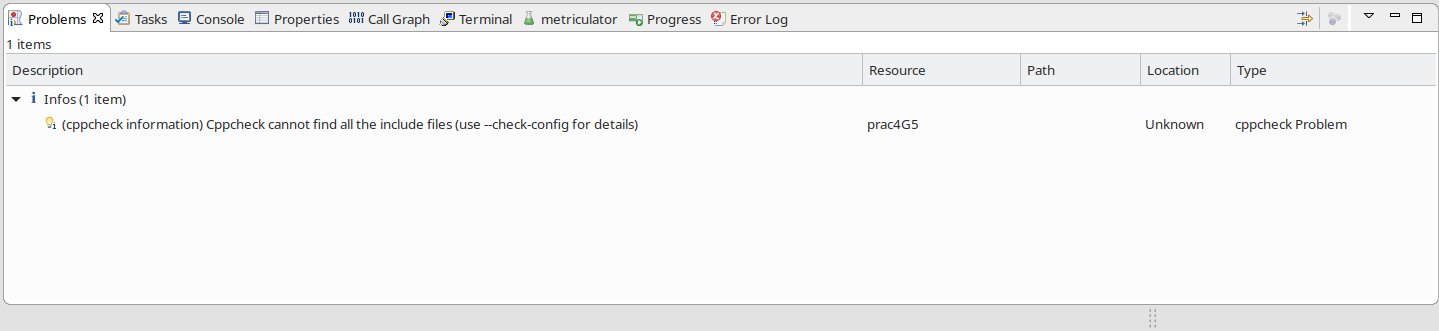
\includegraphics[scale=0.32]{img/captura94.png}
 			\caption{Captura de pantalla de los resultados arrojados tras la ejecución de cppcheck.}
 			\label{captura94}
 		\end{figure}
 	
 		\begin{figure}[H]
 			\centering
 			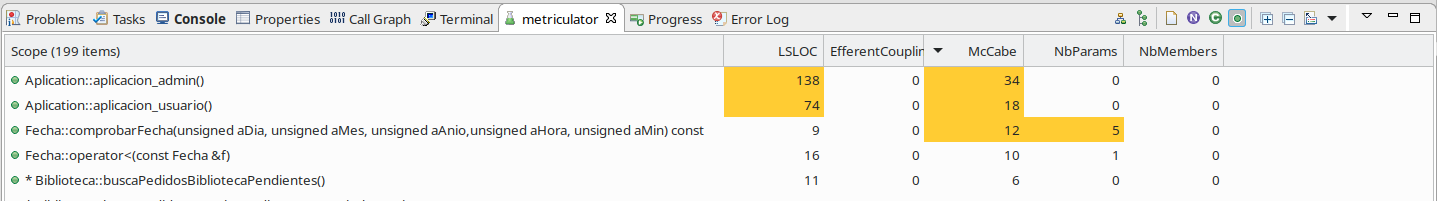
\includegraphics[scale=0.32]{img/captura95.png}
 			\caption{Captura de pantalla de los resultados arrojados tras la ejecución de metriculator.}
 			\label{captura95}
 		\end{figure}
 	
 		\paragraph{}En los resultados arrojados por cppcheck, podemos observar que tenemos un info: no se encuentran todos los includes del proyecto. Tras buscar información, descubrimos que este error es bastante común ya que cppcheck no es capaz de identificar todas las dependencias que son externas a los archivos del proyecto. Por este motivo, y tras revisar que no falla la sintaxis de ninguno de los includes, la forma de resolver este info es simplemente ignorarlo.
 		
 		\paragraph{}Tras solucionar este info, volvemos a ejecutar el análisis de cppcheck y esta vez no nos devuelve ninguna incidencia. A continuación, se muestra una captura de pantalla como justificación.
 		
 		\begin{figure}[H]
 			\centering
 			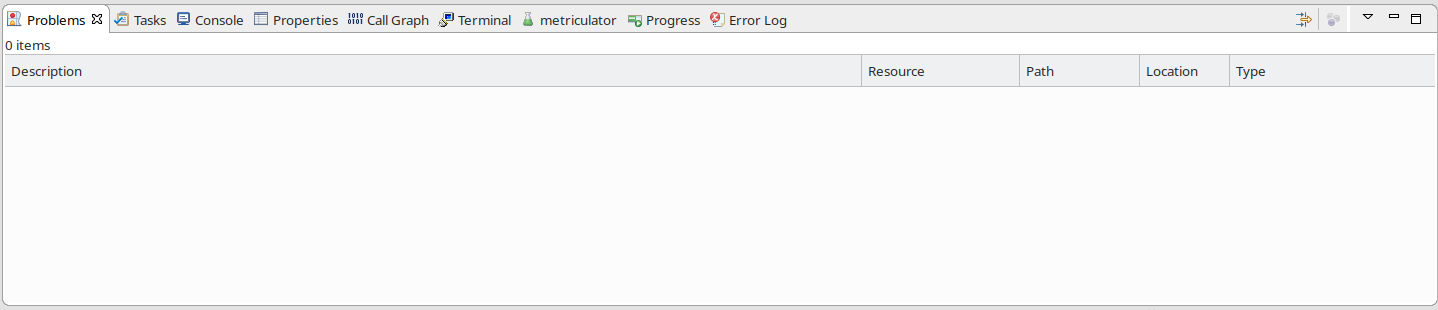
\includegraphics[scale=0.32]{img/captura96.png}
 			\caption{Captura de pantalla de los resultados arrojados tras la ejecución de cppcheck.}
 			\label{captura96}
 		\end{figure}
 	
 		\paragraph{}Respecto a los resultados arrojados por metriculator, podemos observar que aparecen tres módulos que presentan un V(G)$>$10 en la métrica de McCabe:
 		
 		\begin{itemize}
 			\item void Aplication::aplicacion\_admin()
 			\item void Aplication::aplicacion\_usuario()
 			\item void Fecha::comprobarFecha(unsigned aDia, unsigned aMes, unsigned aAnio, unsigned aHora, unsigned aMin) const
 		\end{itemize}
 		
 		
 	\subsection{Corrección del módulo $"void$ $Aplication::aplicacion\_admin()"$}
 	
 		\subsubsection{Estado del módulo antes de la corrección}
 		
 		\paragraph{}Este módulo se encuentra en implementado en la línea 38 del archivo Aplication.cpp del proyecto. Su complejidad ciclomática es de V(G)=34 en la métrica de McCabe. En las siguientes capturas de pantalla se puede observar el estado de dicho módulo antes de realizar las correcciones oportunas.
 		
 		
 		
 		\subsubsection{Estado del módulo después de la corrección}
 		

\newpage